\chapter{Experimental set-up}
\label{ch:experiment}

\section{First: summary of paper}
\subsection{Introduction}

\begin{figure}
\centering
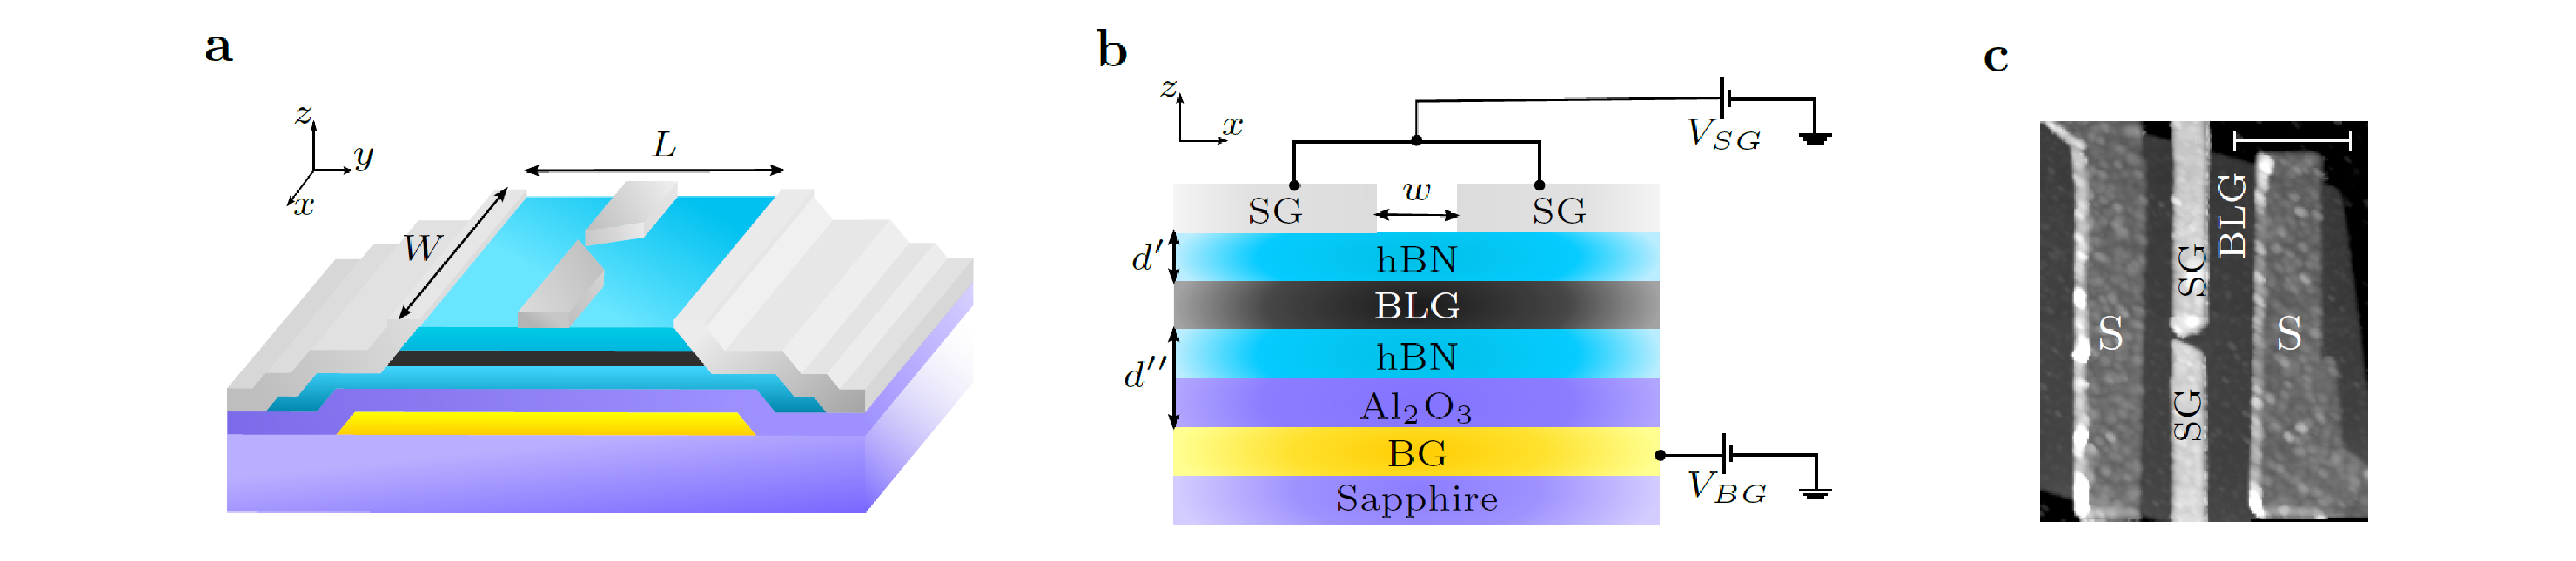
\includegraphics[width=0.8\textwidth]{figure/experiment/setup}
\end{figure}

Josephson effect \cite{Josephson1962} has been studied a lot. Key challenge: Developing devices in which the induced superconductivity can be monitored. This experiment is cool, because it uses local gates to control confinement, amplitude and density profile of the supercurrent. The sample used is a BLG-HBN-VDW heterostructure.
Tunnel barrier -> supercurrent can only be tuned by modifying the geometry/temperature.
Weak link -> a conductive material, in which superconductivity can be induced (proximity effect) and supercurrent can flow over larger distance than in tunnel junction \cite{Likharev1979}.
Magnitude of supercurrent depends on contact transparency, disorder in the weak link, temperature.

Greatness of this work: full control of supercurrent both in amplitude and spatial distribution has not been observed so far. It is difficult to confine charge carriers in graphene (SLG!), because no backscattering in graphene and Klein tunneling \cite{Katsnelson2006}. Using BLG helps, because one can engineer an electronic band gap forming the barrier. 

Sample geometry: QPC-like split gate geometry. The sample is overall gated with a backgate $V_{BG}$, a local top-gate in shape of two fingers (QPC geometry) is used to build a barrier. How does this process work? The overall backgate pushes the fermi level up into the conductance band. The topgate gives a displacement field, it pushes the fermi level down into the band gap --> no conduction possible, insulating state induced.
Asymmetry between the layers of bilyer graphene (different energies at the layer) opens a band gap \cite{McCann2006} that is tuneable.

\subsection*{Normal state analysis:}
\begin{itemize}
\item low charge carrier density $2.8\cdot 10^{18}$.
\item Landau fans in magnetotransport measurement
\item Fabry Perot interferences
\end{itemize}

\subsubsection*{On the resistance maps}
\begin{figure}
\centering
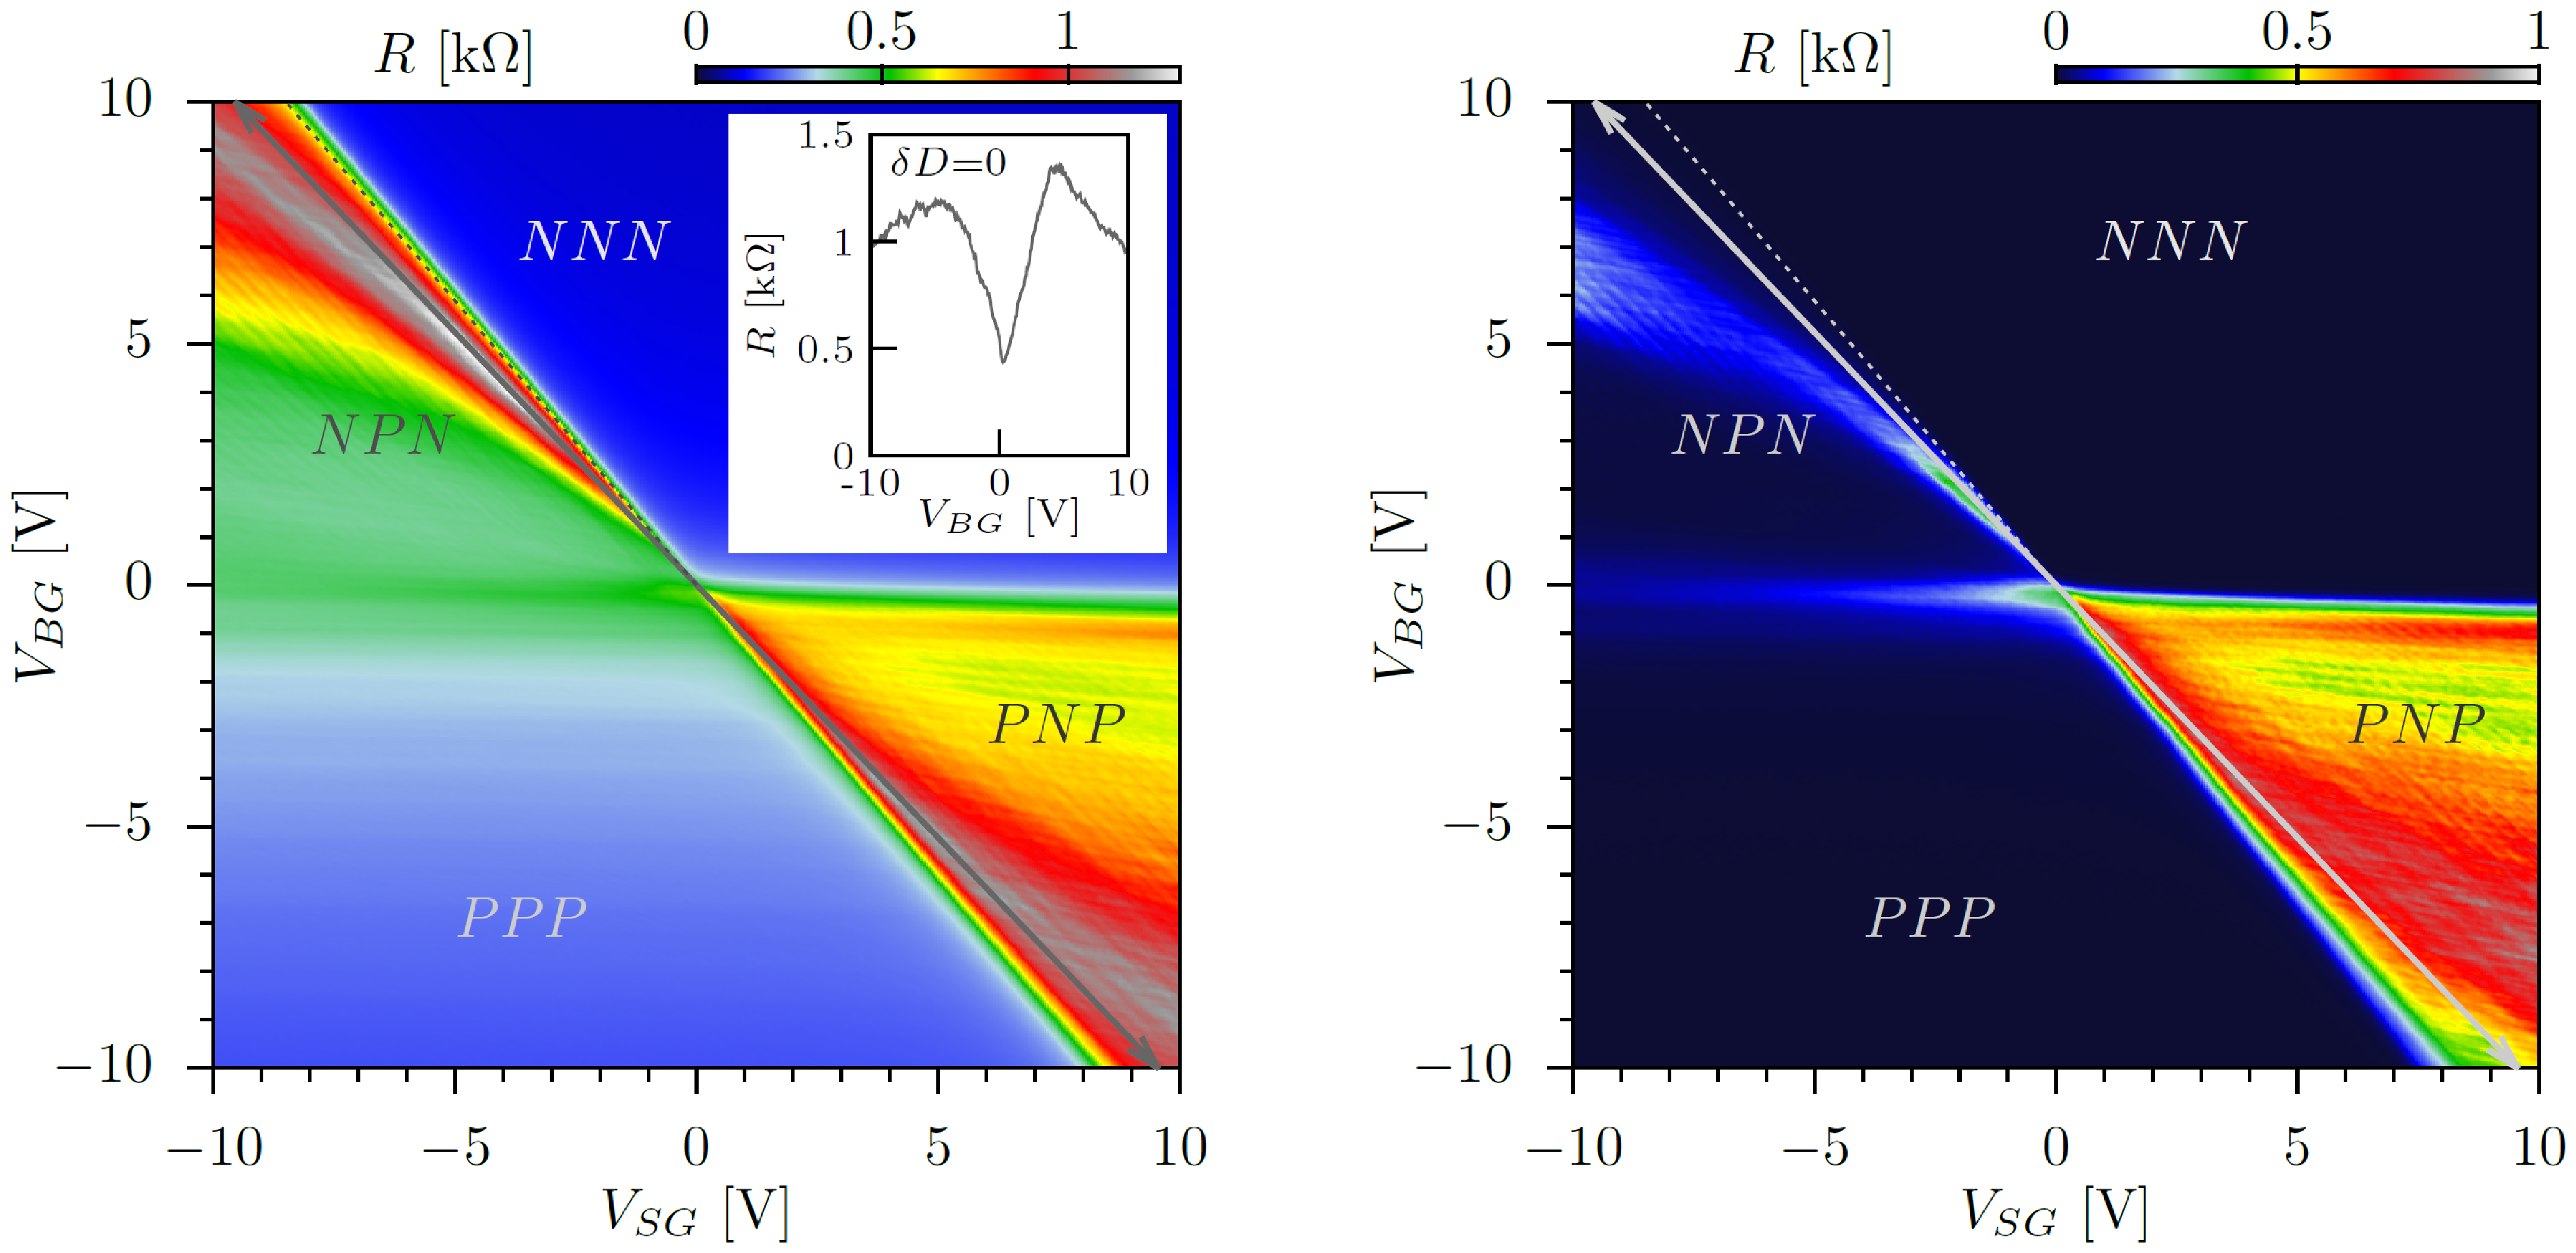
\includegraphics[width=0.8\textwidth]{figure/experiment/resistance-map-edit}
\caption{Resistance maps}
\end{figure}

 The gate map has the backgate as y-axis, the splitgate (QPC topgate) as x-axis and the color indicates the strength of measured resistane. For orientiation, the line where back and splitgate are equal is called the displacement field line (grey arrow). Naming the regions, depending on the position of the fermi level: fermi level in valence band: N, fermi level in conductance band: P. Think of it as three regions: BLG backgated, the area where BLG is back and topgated (region with topgates on top of the material), and again a region where BLG is only backgated. Depending on the the choice of $V_{BG}$ and $V_{SG}$, there are four regions: NNN, NPN, PPP, PNP. Looking at the upper left quadrant, NPN. In this region, the maximum resistance seems to follow the displacement field line (grey arrow), until a certain point, where it bends and the maximum resistance is not on a straight line anymore. Effect is visible in the normal state but even more in the superconducting state. --> unexpected behaviour.
 
Explanation? Charge carrier density is low, the influence of the backgate is important. The higher the backgate value is, the less the charge carrier density is affected by the splitgate and the stray fields, that it produces. And, as the splitgate impact is weak, the device stays conductive (resistance is low) along the displacement field line. 
Why the bending? In the upper region of the displacement field line, the split gates work as intenden: the channel region (the region, where the supercurrent can pass through) is conductive, because the backgate dominates. In the region, where the resistance curve is bending, the stray fields from the splitgate dominate, effectively blocking the channel region and therefore leading to to increased resistance.

The overall resistance is higher on the p-side, due to the slight n-doping of the leads (they create a pn junction at each contact). Can be seen in the supercondcuting state, the pnp region remains resistive, the npn region shows zero resistance.

\subsubsection*{Fabry Perot resonances}

gate dependece of conductance shows oscillatory behaviour, are attributed to Fabry Perot interferences of differenct cavities \cite{Shytov2008}


\subsection*{Superconducting state}
\begin{figure}
\centering
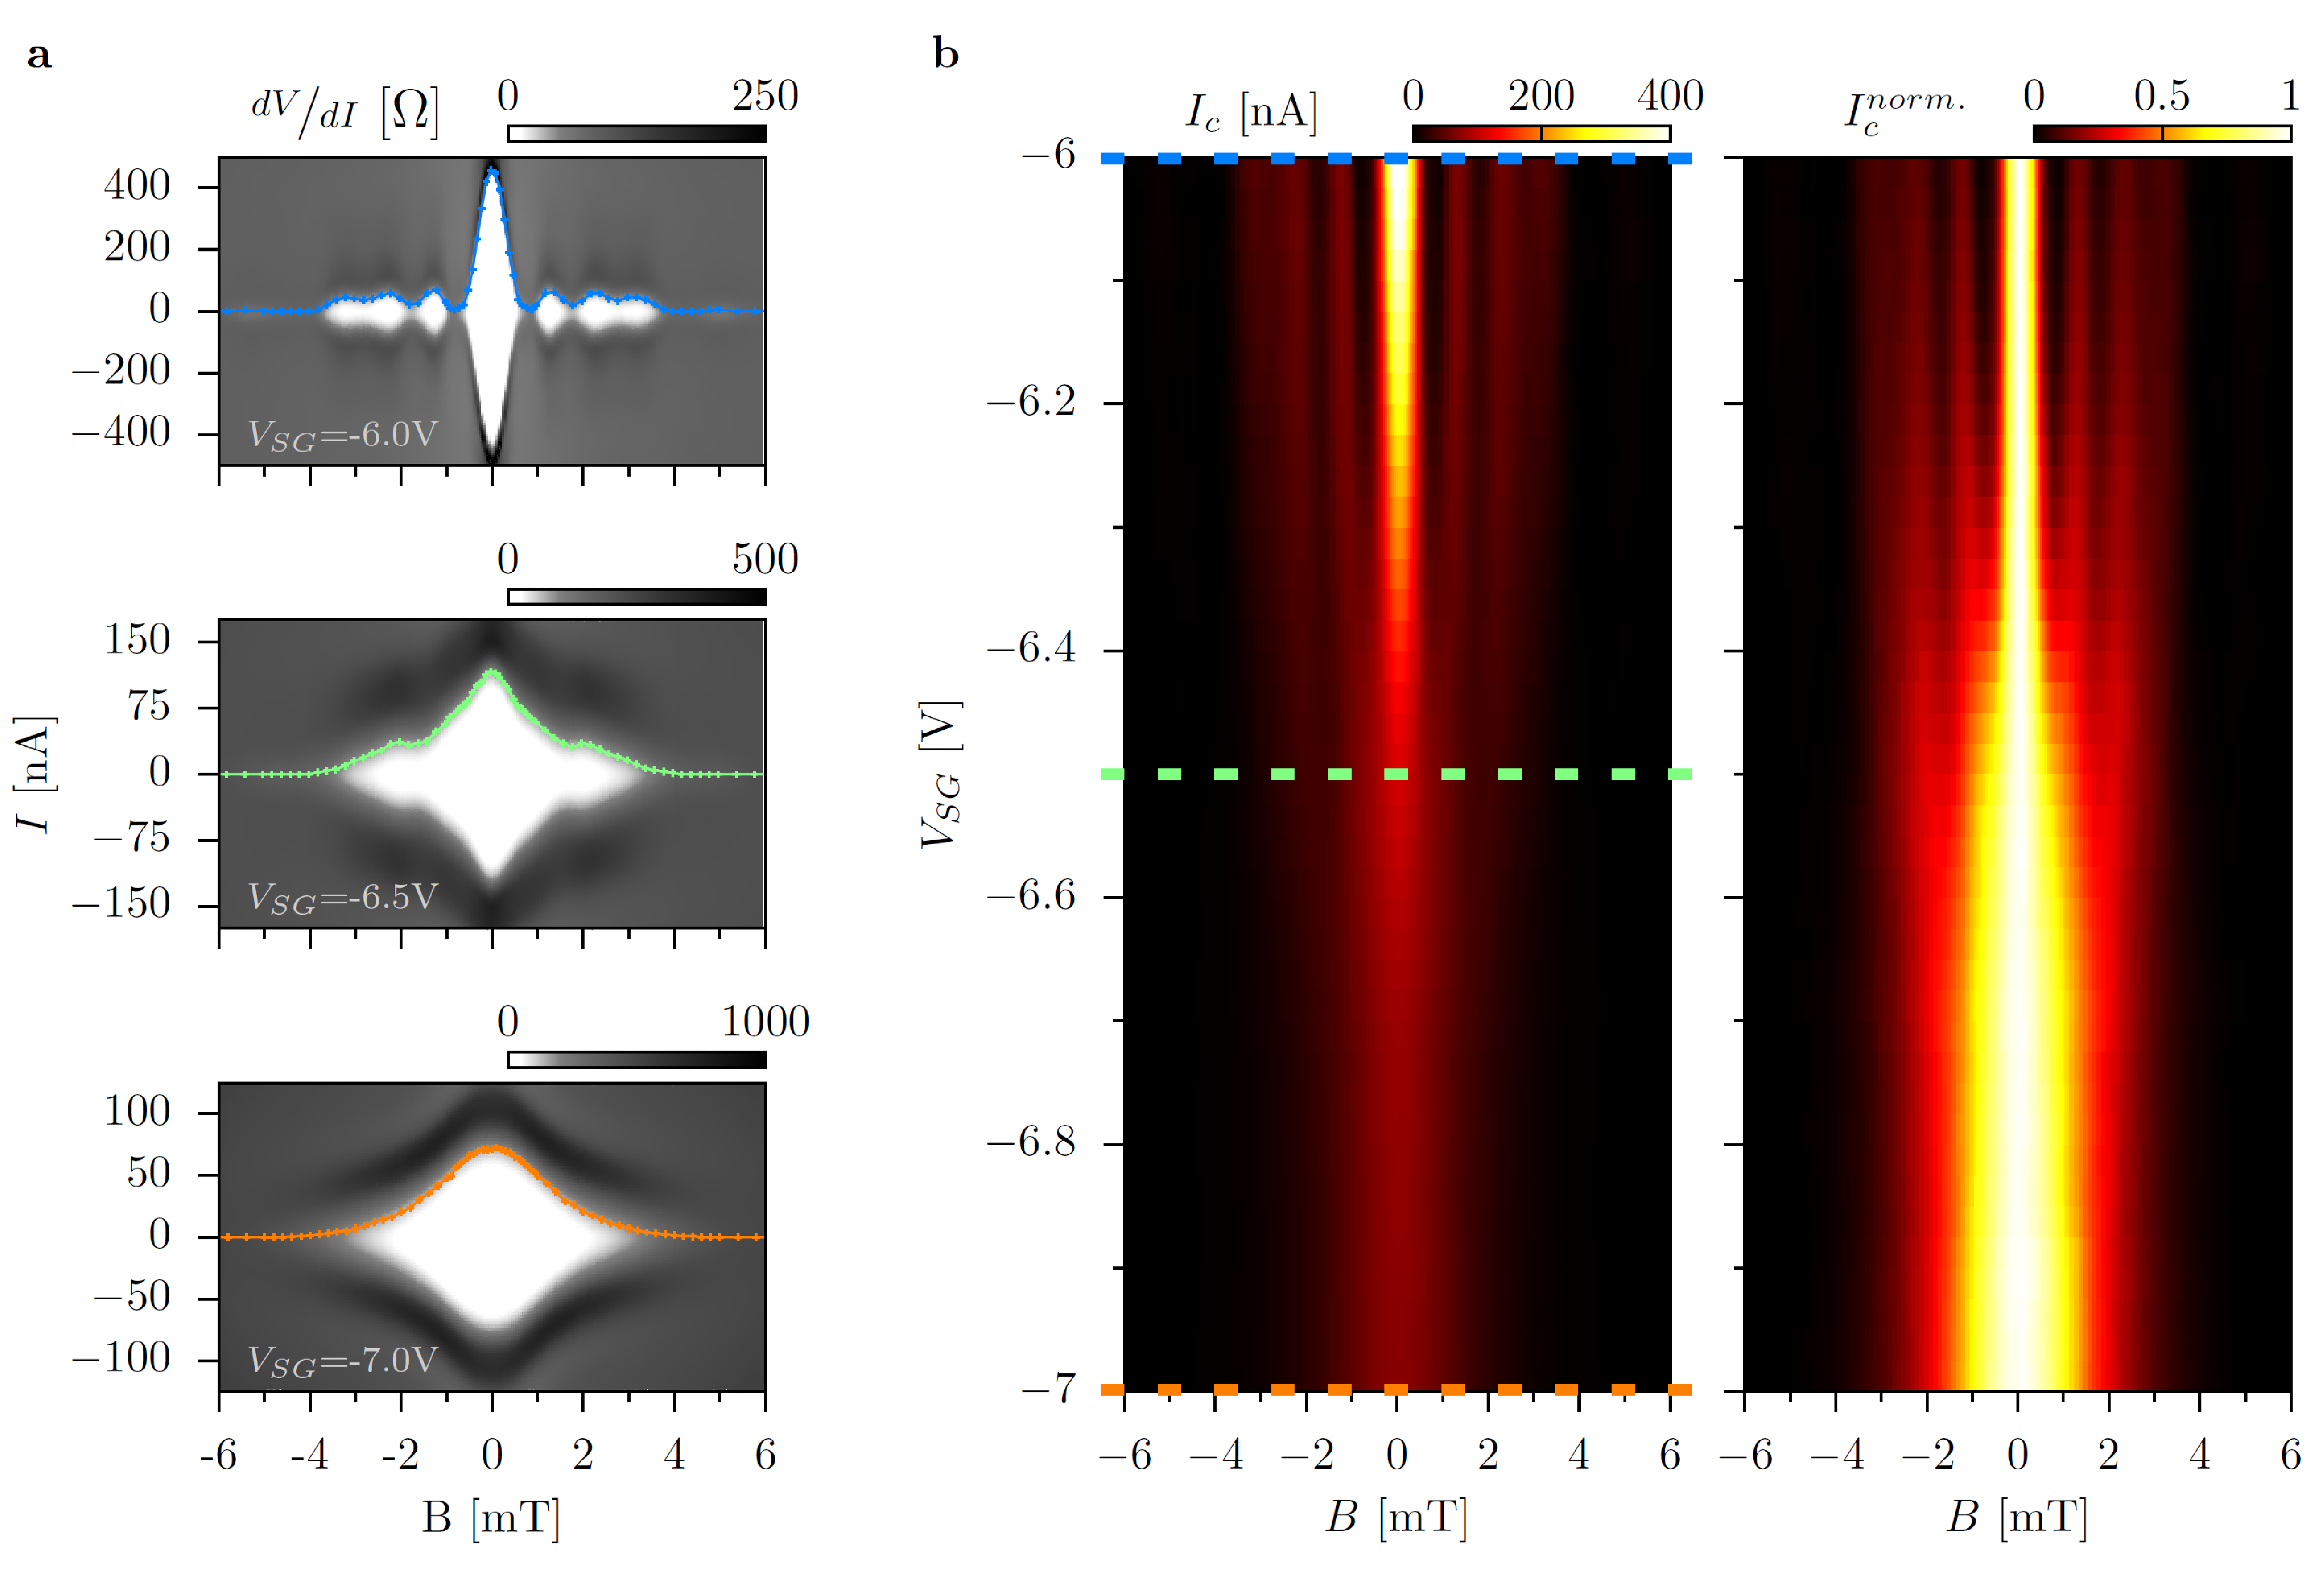
\includegraphics[width=0.8\textwidth]{figure/experiment/supercurrent}
\end{figure}

Since the device becomes superconducting in the npn region, the experiments focus on this part when analysing the supercurrent.

The amplitude of the supercurrent can be monitored by tuning the charge carrier densitiy with the backgate. 

Supercurrent density can be explored by probing the interference pattern in response to a perpendicular magnetic field.  A change of the junction geometry directly manifests within the interference pattern. 

Confinement of the current can be observerd: 
\begin{itemize}
\item open regime: Fraunhofer-like pattern, two dimensional system
\item splitgate increases: lobes are lifted
\item constriction is formed, really a 1D channel has formed: non beating, bell-shaped pattern
\end{itemize}

Transition from Fraunhofer to bell-shaped pattern has been observed before: \cite{Chiodi2012}
